\section{Implementation}

We have implemented Raft as part of LogCabin, a replicated state machine
implemented
as a network service. We initially developed LogCabin to store
configuration information for RAMCloud~\cite{Ousterhout:2011} and assist
in failover of the RAMCloud coordinator. We had planned to implement
Paxos in LogCabin, but the difficulties we faced motivated us to develop
Raft. LogCabin then served as our test platform for new ideas in Raft,
and also as a way to verify that we understood the issues of building a
complete and practical system. The Raft implementation in LogCabin
contains roughly \num{2000} lines of C++ code, not including tests, comments,
or blank lines. The source code is freely available~\cite{logcabin}.
Its architecture is discussed in the next section.

In addition to LogCabin, there are dozens of third-party open-source
implementations of Raft in various stages of
development~\cite{implementations}. Many of these use different
architectures than LogCabin, such as the actor
model~\cite{impl:rafter,impl:akka-raft,impl:archie-raft} or event-based
programming~\cite{impl:kanaka-raft-js,impl:barge,impl:kontiki}. Various
companies are also deploying Raft-based systems~\cite{implementations}.
For example, Facebook is currently testing HydraBase, a fork of Apache
HBase~\cite{HBase}
that uses Raft for replication~\cite{HydraBase}.

\subsection{Threaded architecture}
\label{performance:threads}

\begin{figure}
\centering
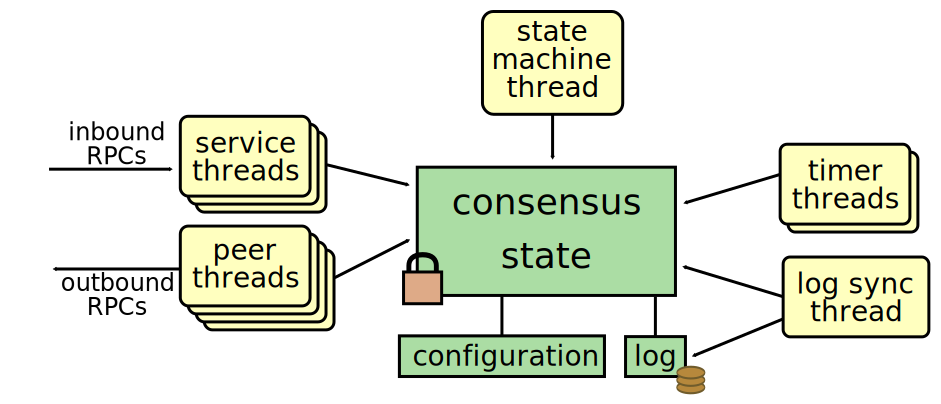
\includegraphics[scale=.4]{performance/threads}
\vcaption[threaded architecture]{
In LogCabin,
consensus state for each server is stored in a monitor protected by a
single lock, accessed by a collection of threads. The threads
communicate with other servers (``peer threads''), handle incoming
requests from clients and other servers (``service threads''), execute
commands in the state machine (``state machine thread''), implement
timeouts (``timer threads''), and write log entries to disk (``log sync
thread'').
}
\label{fig:performance:architecture}
\end{figure}

Raft lends itself to a straightforward implementation architecture using
threads, as shown in Figure~\ref{fig:performance:architecture}. This is
not the only possible architecture, but it is the approach we have taken
in LogCabin. Each server consists of a collection of shared state
variables managed in a monitor style with a single lock.  Five groups of
threads call into the monitor to manipulate the state:
%
\begin{itemize}
%
\item \textbf{Peer threads:} 
%
There are as many peer threads as there are other servers in the
cluster; each peer thread manages the RPCs to one of the other servers.
Each thread enters the consensus state monitor, using a condition
variable to wait for events that require communication with the given
server. Then it leaves the monitor (releasing the lock) and issues an
RPC. Once the RPC completes (or fails), the peer thread reenters the
consensus state monitor, updates state variables based on the RPC, and
waits for the next event that requires communication.
%
\item \textbf{Service threads:}
%
Several threads handle incoming requests from clients and other servers.
These threads wait outside the consensus state monitor for incoming
requests, then enter the monitor to carry out each request.
%
\item \textbf{State machine thread:}
%
One thread executes the state machine. It enters the consensus state
monitor to wait for the next committed log entry; when an entry is
available, it leaves the monitor, executes the command, and returns to
the monitor to wait for the next command.
%
\item \textbf{Timer threads:}
%
One thread manages the election timer for both followers and candidates;
it starts a new election once a randomized election timeout has elapsed.
A second thread causes the server to return to the follower state if, as
leader, it is unable to communicate with a majority of the cluster;
clients are then able to retry their requests with another server (see
Section~\ref{clients:findleader}).
%
\item \textbf{Log sync thread:} When the server is leader, one thread
writes log entries durably to disk. This is done without holding the
lock on the consensus state, so replication to followers can proceed in
parallel; see Section~\ref{performance:leaderdisk}. For simplicity,
followers and candidates write directly to disk from their service
threads while holding the consensus lock; they do not use the log sync
thread.
%
\end{itemize}
